%\documentclass[10pt]{beamer} %with transitions 
\documentclass[handout, 10pt]{beamer}  %without transitions
\usepackage[utf8]{inputenc}

\setbeamertemplate{note page}[plain]
%\setbeameroption{show notes} 

\setbeamertemplate{footline}[frame number]

\usepackage[style = phys]{biblatex}
\addbibresource{biblio.bib}


\makeatletter
\long\def\beamer@@ssection*#1{\beamer@section[]{}}
\makeatother

\usepackage{physics}

\usepackage{amsmath}
\usepackage{tikz}
\usetikzlibrary{tikzmark}
\setbeamertemplate{caption}[numbered]

\newcommand{\nl}{\\ \vspace{1em}}

\mode<presentation> {

% The Beamer class comes with a number of default slide themes
% which change the colors and layouts of slides. Below this is a list
% of all the themes, uncomment each in turn to see what they look like.

%\usetheme{default}
%\usetheme{AnnArbor}
%\usetheme{Antibes}
%\usetheme{Bergen}
%\usetheme{Berkeley}
%\usetheme{Berlin}
%\usetheme{Boadilla}
%\usetheme{CambridgeUS}
%\usetheme{Copenhagen}
%\usetheme{Darmstadt}
%\usetheme{Dresden}
%\usetheme{Frankfurt}
%\usetheme{Goettingen}
%\usetheme{Hannover}
\usetheme{Ilmenau}
%\usetheme{JuanLesPins}
%\usetheme{Luebeck}
%\usetheme{Madrid}
%\usetheme{Malmoe}
%\usetheme{Marburg}
%\usetheme{Montpellier}
%\usetheme{PaloAlto}
%\usetheme{Pittsburgh}
%\usetheme{Rochester}
%\usetheme{Singapore}
%\usetheme{Szeged}
%\usetheme{Warsaw}

% As well as themes, the Beamer class has a number of color themes
% for any slide theme. Uncomment each of these in turn to see how it
% changes the colors of your current slide theme.

%\usecolortheme{albatross}
%\usecolortheme{beaver}
%\usecolortheme{beetle}
%\usecolortheme{crane}
%\usecolortheme{dolphin}
%\usecolortheme{dove}
%\usecolortheme{fly}
%\usecolortheme{lily}
%\usecolortheme{orchid}
%\usecolortheme{rose}
%\usecolortheme{seagull}
%\usecolortheme{seahorse}
%\usecolortheme{whale}
%\usecolortheme{wolverine}

%\setbeamertemplate{footline} % To remove the footer line in all slides uncomment this line
%\setbeamertemplate{footline}[page number] % To replace the footer line in all slides with a simple slide count uncomment this line

%\setbeamertemplate{navigation symbols}{} % To remove the navigation symbols from the bottom of all slides uncomment this line
}

\usepackage{multicol} %used for multiple columns

\usepackage{graphicx} % Allows including images
\usepackage{booktabs} % Allows the use of \toprule, \midrule and \bottomrule in tables

\usepackage{braket} %quantum brackets



%----------------------------------------------------------------------------------------
%	TITLE PAGE
%----------------------------------------------------------------------------------------

\title[A Toy Model of Quantum Gravity]{Canonical Quantization Procedure and \\ Time-Energy Uncertainty} % The short title appears at the bottom of every slide, the full title is only on the title page
\subtitle{A Toy Model of Quantum Gravity}
\author[Daniel Prelipcean]{Daniel Prelipcean} % Your name
\institute[JUB Physics BSc Thesis Colloquium] % Your institution as it will appear on the bottom of every slide, may be shorthand to save space
{Physics BSc Thesis Colloquium}
\date{May 16$^{th}$, 2018} % Date, can be changed to a custom date



\begin{document}

\begin{frame}
\titlepage % Print the title page as the first slide

\begin{figure}[H]
  \centering
  \begin{minipage}[H]{0.59\textwidth}
    \raggedright
    
    {\small Supervisor: Prof. Dr. Peter Schupp\\
    2$^{nd}$ Reader: Prof. Dr. S{\"o}ren Petrat }
  \end{minipage}
  \hfill
  \begin{minipage}[H]{0.39\textwidth}
    \raggedleft
    \includegraphics[width=0.75\textwidth]{Figs/JACOBS_LOGO.jpg}
\end{minipage}
\end{figure}




\end{frame}



%----------------------------------------------------------------------------------------
%	PRESENTATION SLIDES
%----------------------------------------------------------------------------------------

%------------------------------------------------
\section{Introduction} % Sections can be created in order to organize your presentation into discrete blocks, all sections and subsections are automatically printed in the table of contents as an overview of the talk


%===================================================


\begin{frame}
\frametitle{The Time-Energy Uncertainty Relation}

First postulated by Heisenberg \cite{HeisenbergUR}, the Time-Energy Uncertainty is:

\begin{equation}
\tikzmark{a}\Delta E \cdot  \tikzmark{b}\Delta t  \geq \hbar/2
\end{equation}
\begin{tikzpicture}[remember picture,overlay]

\uncover<3->{
\draw[<-] 
  ([shift={(12pt,-2pt)}]pic cs:a) |- ([shift={(+2pt,-10pt)}]pic cs:a) 
  node[anchor=east] {\small Hamiltonian $\hat{H}$ eigenvalue}; 
  %first pair (x,y) is the shift of the position
  %second pair (x,y) is the size of the arrow
}  
\only<4->{
\draw[<-] 
  ([shift={(11pt,-2pt)}]pic cs:b) |- ([shift={(32pt,-10pt)}]pic cs:b) 
  node[anchor=west] {\small ?}; }
 
\end{tikzpicture}

\uncover<2->{
\begin{alertblock}{Problem 1: No self-adjoint time operator}
No axiomatic derivation similar $\Delta \hat{x} \cdot \Delta \hat{p} \geq \hbar/2$ based on their commutation relation $[\hat{x}, \hat{p}] = i \hbar$, since a time operator $\hat{t}$ does not exist.
\end{alertblock}
}

\uncover<5->{
\begin{alertblock}{Problem 2: Different interpretations of time uncertainty}
\begin{enumerate}
\uncover<6->{\item Energy-dispersion ($\Delta E$) of a state and its lifetime ($\Delta t$) }

\uncover<7->{\item Energy exchange ($\Delta E$) and exchange time-frame ($\Delta t$) }

\uncover<8->{\item Energy measurement ($\Delta E$) and measurement/preparation time ($\Delta t$)}
\end{enumerate}

\end{alertblock}
}



\end{frame}

%===================================================





%=====================================================
\section{Theory: Reinterpretation}








%=====================================================

\begin{frame}
\frametitle{Notation and Klein-Gordon equation}

Notation:
\begin{enumerate}
\uncover<2->{\item four vectors: $x^\mu = (t, \vec{x})$ and $p^\mu = (E, \vec{p})$}
\uncover<3->{\item Minkowski metric: $\eta_{\mu\nu} = (-, +,+,+)$}
\uncover<4->{\item Einstein summation convention: $p_\mu p^\mu = p_\mu p_\nu \eta^{\mu\nu} = - p_0^2 + \vec{p} \ ^2$}
\end{enumerate}


\uncover<5->{\textit{Def:} A constraint on a system is a dynamical relation that the system must obey, of the form:
\begin{equation}
 \phi (x^\mu,p_\mu)=0
\end{equation}}
\uncover<6->{e.g. the mass-shell constraint:
\begin{equation}
p_\mu p^\mu + m^2c^2 =0
\end{equation}}
\uncover<7->{For $\hat{p}_\mu = -i \hbar \partial_\mu$,} \uncover<8->{ quantizing the above yields:
\begin{equation}
\left( \hat{p}_\mu \hat{p}^\mu + m^2c^2 \right) \ket{\psi}= (- \hbar^2 \partial_\mu \partial^\mu +m^2c^2 )\ket{\psi} =0
\end{equation}}
\uncover<9->{i.e. the Klein-Gordon equation.}
\end{frame}


%=====================================================

\begin{frame}


\frametitle{Free Relativistic Bosonic Particle}
\uncover<2->{The Hamiltonian after quantizing the simplest example is:
\begin{equation}
    \hat{H} (x^\mu, p_\mu) \ket{\psi} = \frac{1}{2} (\hat{p}_\mu \hat{p}^\mu + m^2_{ }c^2) \ket{\psi}=  0
\end{equation}}
\uncover<3->{This is called a Hamiltonian Constraint.}

\uncover<4->{\begin{alertblock}{ \uncover<2->{Problem of Time in Quantum Gravity}}
\begin{equation}
    \uncover<5->{i \hbar \frac{\partial}{\partial t} \ket{\psi}} \uncover<6->{ = \hat{H} \ket{\psi}} \uncover<7->{ = 0 }
\end{equation} 
\end{alertblock}}

\uncover<8->{
\begin{block}{Proposed solution: $4 +1$ formalism}
Introduce an extra parameter time $\lambda$ giving the system's evolution as:
\begin{equation}
 i\hbar \dfrac{\partial}{\partial \lambda} \ket{\psi}\uncover<9->{ = \hat{H}_0 \ket{\psi}}
\end{equation}
\end{block}}


\end{frame}

%=====================================================


\begin{frame}
\frametitle{World Line Parametrization}


 \begin{columns}

  \column{0.45\linewidth}
  
\uncover<3->{An observer moves in space-time as parametrized by the time evolution parameter $\lambda$. \cite{Pavsic}}
\vspace{1em}

\uncover<4->{e.g. identify the parameter with proper time:
\begin{equation}
\lambda = \alpha \tau
\end{equation}}

\uncover<5->{Just a specific gauge choice, in general, $\lambda = f(\tau)$.}


  \column{0.45\linewidth}
  \centering
\uncover<2->{ 
\begin{figure}
  \centering
 \includegraphics[width=0.8\textwidth]{Figs/Space_Time_Diagrams.pdf}
  \centering
  \caption{World line parametrization by $\lambda$}
  \label{fig:b} 
  \end{figure}
}
  \end{columns} 
\end{frame}

%=====================================================
\begin{frame}


\frametitle{Free Relativistic Bosonic Particle (Again)}
The Hamiltonian constraint after quantizing the simplest example is:
\begin{equation}
    \hat{H} \ket{\psi}\uncover<5->{_{m}} = \frac{1}{2} ( \underbrace{\hat{p}_\mu \hat{p}^\mu}_{\text{operator}} + \underbrace{m^2_{ }c^2}_{\text{scalar value}}) \ket{\psi}\uncover<5->{_{m}} =  0
\end{equation}

\uncover<2->{Reinterpret as parameter time independent equations:}

\uncover<3->{
\begin{equation}
 \hat{H}_0 \ket{\psi}\uncover<5->{_{m}} =  \hat{p}_\mu \hat{p}^\mu  \ket{\psi}\uncover<5->{_{m}} =  i \hbar \dfrac{\partial }{\partial \lambda}\ket{\psi}\uncover<5->{_{m}} \uncover<4->{ \stackrel{!}{=}   - m^2c^2 \ket{\psi}}\uncover<5->{_{m}}
    \label{parameternergyeigenvalueeqn}
\end{equation}
}
\uncover<5->{
solved by physical wave functions $\ket{\psi}_m \in \mathcal{H}_m \subset \mathcal{H}$.}\\

\uncover<6->{But for arbitrary (not necessary on mass-shell) wave functions:}
\uncover<7->{
\begin{block}{Parameter time evolution}
\begin{equation}
\hat{H}_0 \ket{\psi} = \hat{p}_\mu \hat{p}^\mu \ket{\psi}=   i\hbar \dfrac{\partial \ket{\psi}}{\partial \lambda}
\end{equation}}
\end{block}




\end{frame}
\section{Results}

%=====================================================


\begin{frame}
\frametitle{Extension to Four Coordinate Dimensions}

\uncover<2->{The wave functions $\ket{\psi}$ live in a four dimensional Hilbert Space, taken to be $\mathcal{H} = L^2(\mathbb{R}^4)$.}

\uncover<3->{
\begin{equation}
    \langle \psi _{1}|\psi _{2}\rangle = \int_{\mathbb{R}^4} {\mathrm  {d}}^4 x \, \psi _{1}^{\ast }(x^\mu) \psi_{2}(x^\mu)  \quad \text{with} \quad  \norm{\psi} = \sqrt{\braket{\psi|\psi}} \leq \infty
    \label{def:innerproduct}
\end{equation}
}
\uncover<4->{
\begin{alertblock}{Problem: How to normalize wave functions in time?}

\uncover<5->{Take $U(t) = \exp{ -i E t} $, then any wave function would be non-normalizable, as:
\begin{equation}
\braket{\psi|\psi} = \int_{\mathbb{R}} dt  U^{\ast}(t) U(t)\int_{\mathbb{R}^3} {\mathrm  {d}}^3 x \, \psi^{\ast }(\vec{x}) \psi(\vec{x}) = \uncover<6->{\int_{\mathbb{R}} dt } \uncover<7->{\to \infty}
\end{equation}}
\end{alertblock}
}
\begin{center}
\uncover<8->{\textbf{Time Gaussian Wave Packets!}}
\end{center}




\end{frame}

%=====================================================
\begin{frame}

\frametitle{Time-localized Wave Functions}

\uncover<2->{
\begin{block}{Particles localized in time}
Wave packets evolve in parameter time $\lambda$ and propagate in the space-time.
\end{block}
}

\begin{figure}[ht]
        \begin{minipage}[b]{0.54\linewidth}
\uncover<3->{             \centering
            \includegraphics[width=1.00\textwidth]{Figs/LightCones_PosDisl.PNG}
            \caption{Space-time probabilities}
            \label{fig:a}}
        \end{minipage}
        \hfill
        \begin{minipage}[b]{0.44\linewidth}
\uncover<4->{             \centering
            \includegraphics[width=1.00\textwidth]{Figs/GaussianSpread.PNG}
            \caption{Gaussian Spreading \cite{Pavsic}}
            \label{fig:b}}
        \end{minipage}
\end{figure}


\end{frame}



%=====================================================
\begin{frame}
\frametitle{Probability Interpretation}
The Born probability interpretation \cite{Born} holds! \uncover<2->{By construction, the probability density $\rho = \psi^* \psi$ is positive and moreover:}
\uncover<3->{
\begin{block}{Continuity equation}
\begin{equation}
 \uncover<4->{\partial_\lambda \rho + } \partial_\mu j^\mu = 0
\end{equation}
\end{block}
  }
 \uncover<5->{
where:
\begin{equation}
j^\mu = - i  ( \psi^* \partial^\mu \psi -  \psi \partial^\mu \psi^*)
\end{equation}
}
\end{frame}


%=====================================================
\begin{frame}
\frametitle{Time-Energy Uncertainty}
 \uncover<2->{
Uncertainty relations \cite{RobertsonUR} for operators $\hat{A}$ and $\hat{B}$:}
 \uncover<3->{
\begin{equation}
 (\Delta{\hat{A}})^{2}(\Delta{\hat{B}})^{2}\geq \frac {1}{2} \left|\langle [{\hat {A}},{\hat {B}}]\rangle \right|^{2}  
\end{equation}
}
\uncover<4->{From the position-momentum commutation relation $[\hat{x}^\mu, \hat{p}_\nu] = i \hbar \delta^\mu_\nu $:
\begin{equation}
    \Delta \hat{x}^{\mu} \Delta \hat{p}_{\nu} \geq \frac{1}{2} \left|  \bra{\psi} \left[ \hat{x}^\mu, \hat{p}_\nu \right] \ket{\psi} \right| = \frac{ \hbar}{2} \delta_\nu^\mu 
\end{equation} 
}
 \uncover<5->{The zeroth component is:}
 \uncover<6->{
\begin{block}{Main result: The Time-Energy Uncertainty}
\begin{equation}
\Delta x^{0} \Delta p_{0} = \Delta t \Delta E \geq \frac{ \hbar}{2}
\end{equation}
\end{block}
}

\end{frame}


\section{Conclusion}
%=====================================================
\begin{frame}
\frametitle{Summary}
\begin{enumerate}
\uncover<2->{\item Introduced another time evolution parameter $\lambda$ to implement the Hamiltonian constraint as an eigenvalue problem.}
\uncover<3->{\item Promoted coordinate time $t = x^0$ to an operator.}
\uncover<4->{\item Reformulated  Relativistic Quantum Mechanics for the Bosonic Free Particle accordingly: $\psi \in L^2(\mathbb{R}^4)$, probability interpretation, etc.}
\uncover<5->{\item Axiomatically obtained the Time-Energy Uncertainty Relation via operator commutation relations.}
\end{enumerate}



\end{frame}


%=====================================================



\section*{References}
\begin{frame}
\frametitle{References}
\printbibliography
\end{frame}

%=====================================================

\iffalse
\section{Post Scriptum}

\begin{frame}
\frametitle{Stages of the Research Process}
\begin{enumerate}
\pause \item Identify and develop topic
\pause \item Find Background Information
\pause \item Obtain new results that you are very excited about
\pause \item Realize someone else has already done the same 
\end{enumerate}

\end{frame}
%=====================================================

\begin{frame}
\begin{block}{New Results}
Mention of and focus on the time-energy uncertainty.\\
Different interpretation of constraints as parameter time independent.\\
General parameter $\lambda$ rather than just proper time.\\

\end{block}

\end{frame}
\fi

\end{document}